\documentclass[english,11pt,a4paper]{article}
\usepackage[T1]{fontenc} % --------------| More characters.
\usepackage[utf8]{inputenc} % -----------| Direct use of scandinavian letters.
\usepackage{float} % --------------------| More options for floats.
\usepackage{graphicx} % -----------------| Support more image formats.
\usepackage{booktabs} % -----------------| Better-looking tables.
\usepackage{tabularx} % -----------------| Better tables
\usepackage{subcaption} % ---------------| Subfigures.
\usepackage[a4paper]{geometry} % --------| Adjusting page margins.
\usepackage{amsmath,amssymb,amsfonts} % -| Various math, including eqref.
\usepackage{xcolor} % -------------------| Allows defn. of custom colors.
\usepackage{babel}
\usepackage{url}
\usepackage{enumitem}

% XY-pic. Used for creating illustrations.
\input xy
\xyoption{all}

% Styling captions.
\usepackage{caption}
\captionsetup{margin=10pt,font=small,labelfont=bf}



\begin{document}

\title{Reservoir Simulation, Exercise 1}
\author{Einar Baumann}
\maketitle
\thispagestyle{empty}
\pagebreak

\section{Derivation of the numerical solutions for the linear flow PDE} % (fold)
\label{sec:derivation}
Starting with the PDE for linear flow:

\begin{equation}
  \frac{\partial^2 P}{\partial x^2} = \frac{\phi \mu c}{k} \frac{\partial P}{\partial t}
\end{equation}

For the later discretization we will use a \emph{block-centered grid} to divide the \emph{x}- and \emph{t}-coordinates into discrete grid blocks. The pressure in each block will then be solved numerically for each block for each time step. 

\begin{xy}
  (0,5)*+{1};%
  (0,0)*+{\bullet} **\frm{-}
\end{xy}

% section derivation (end)
\pagebreak


\section{FORTRAN program} % (fold)
\label{sec:fortran_program}

\subsection{Plots} % (fold)
\label{sub:plots}

\begin{figure}[H]
  \centering
  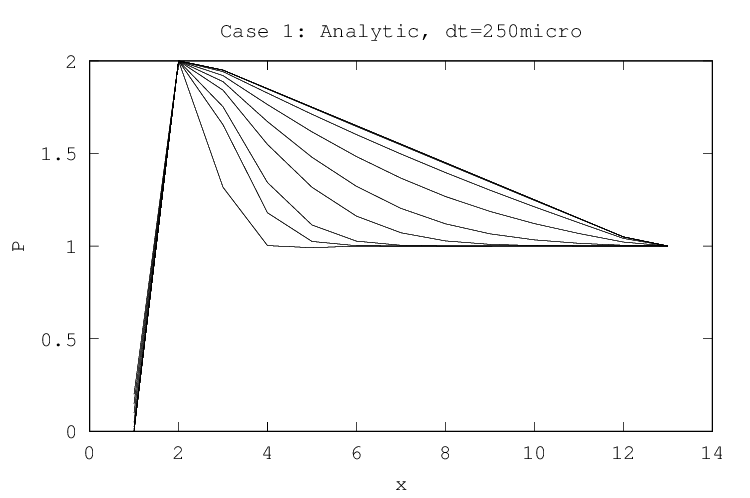
\includegraphics[]{../code/case1.png}
  \caption{Case 1.}
  \label{fig:case1}
\end{figure}

\begin{figure}[H]
  \centering
  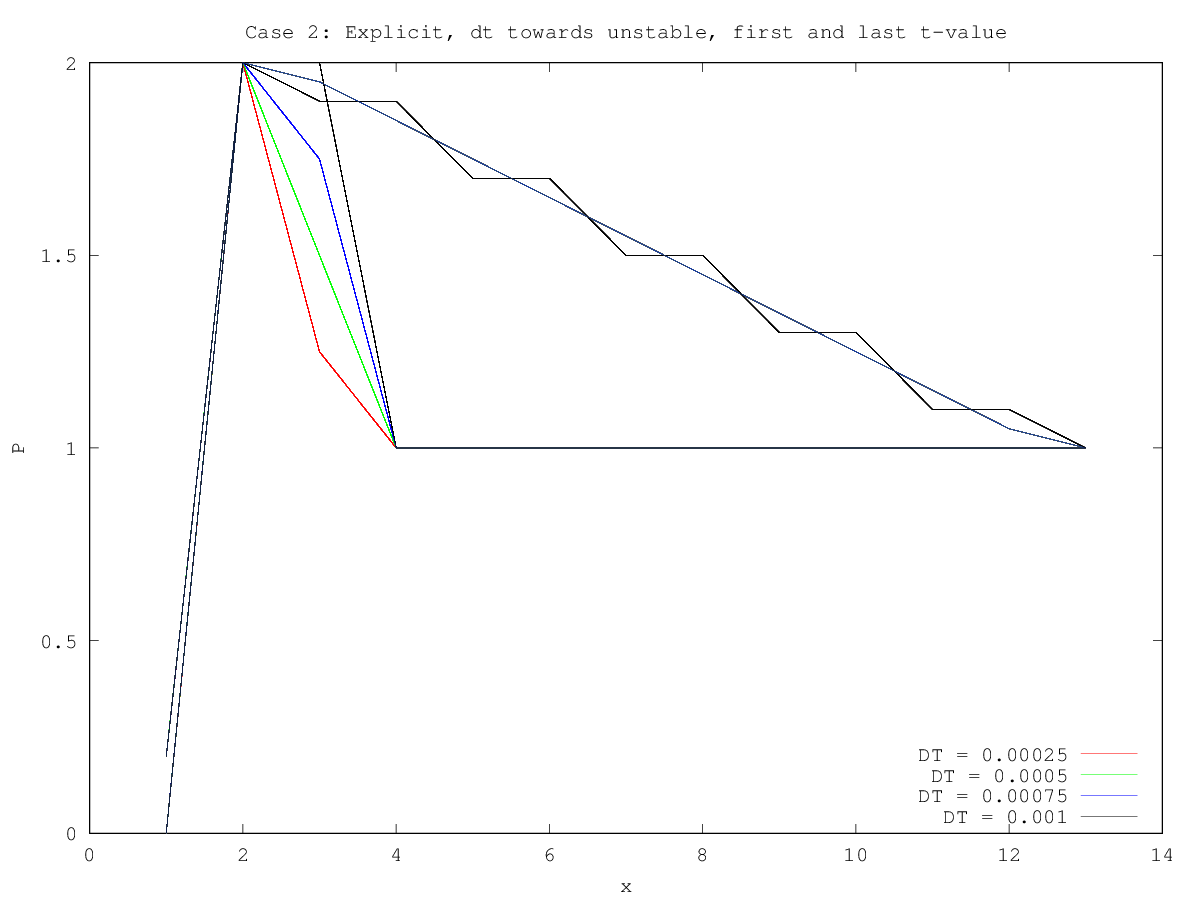
\includegraphics[]{../code/case2.png}
  \caption{Case 2.}
  \label{fig:case2}
\end{figure}

\begin{figure}[H]
  \centering
  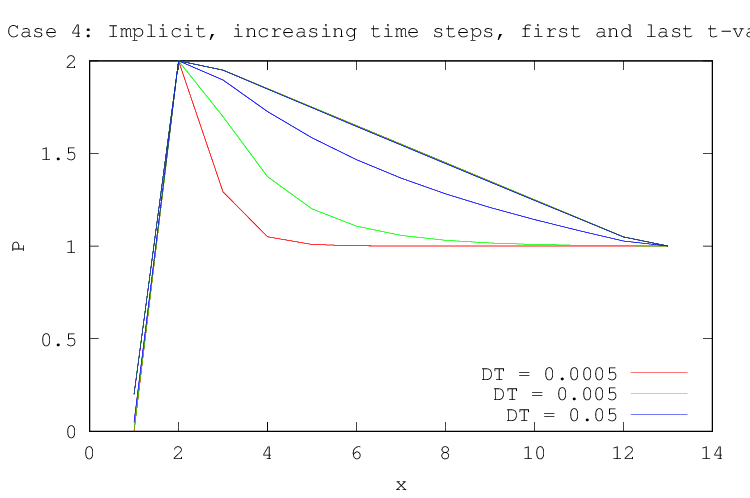
\includegraphics[]{../code/case4.png}
  \caption{Case 4.}
  \label{fig:case4}
\end{figure}

\begin{figure}[H]
  \centering
  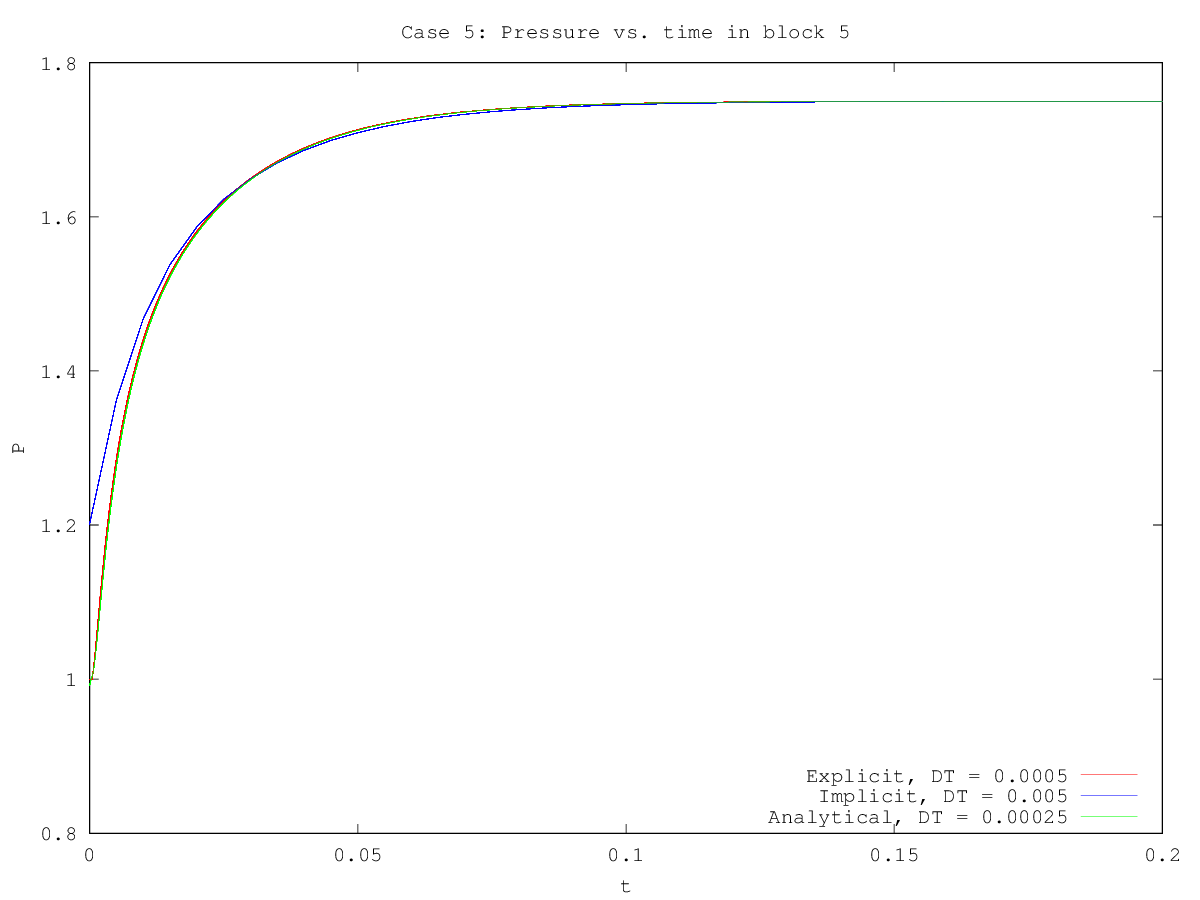
\includegraphics[]{../code/case5.png}
  \caption{Case 5.}
  \label{fig:case5}
\end{figure}

\begin{figure}[H]
  \centering
  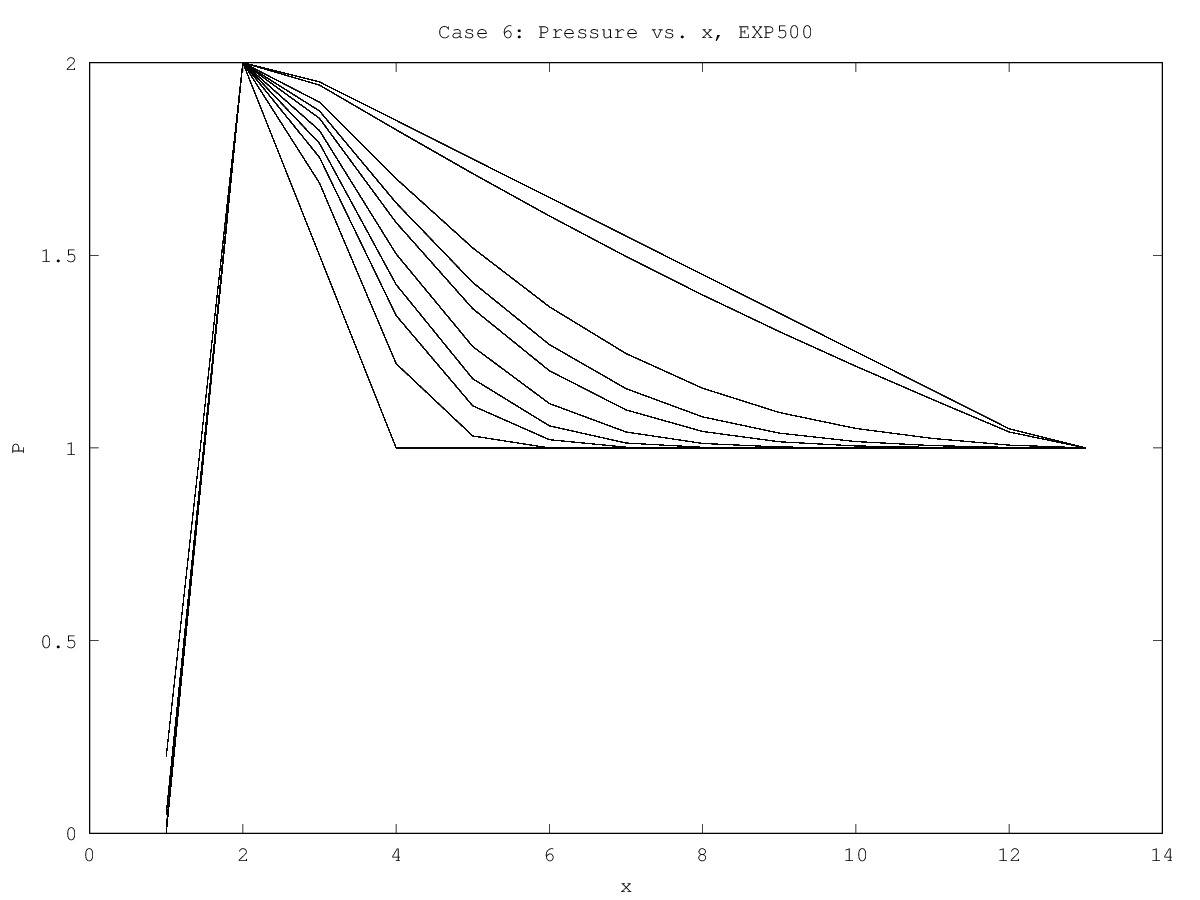
\includegraphics[]{../code/case61.png}
  \caption{Case 6, explicit solution.}
  \label{fig:case61}
\end{figure}

\begin{figure}[H]
  \centering
  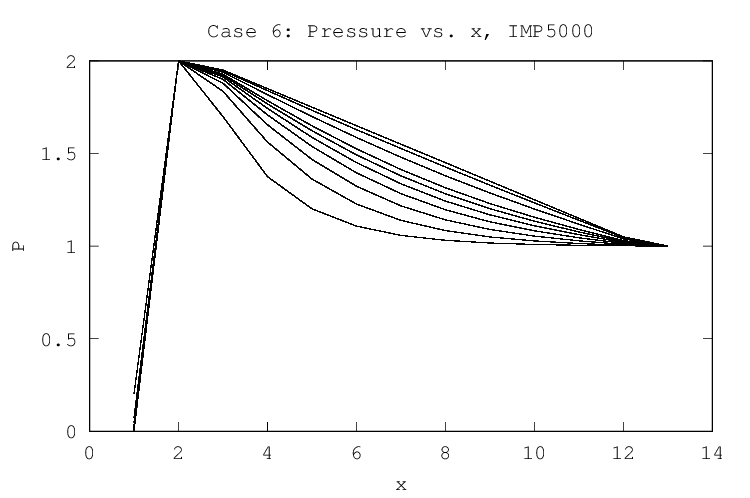
\includegraphics[]{../code/case62.png}
  \caption{Case 6, implicit solution.}
  \label{fig:case62}
\end{figure}

\begin{figure}[H]
  \centering
  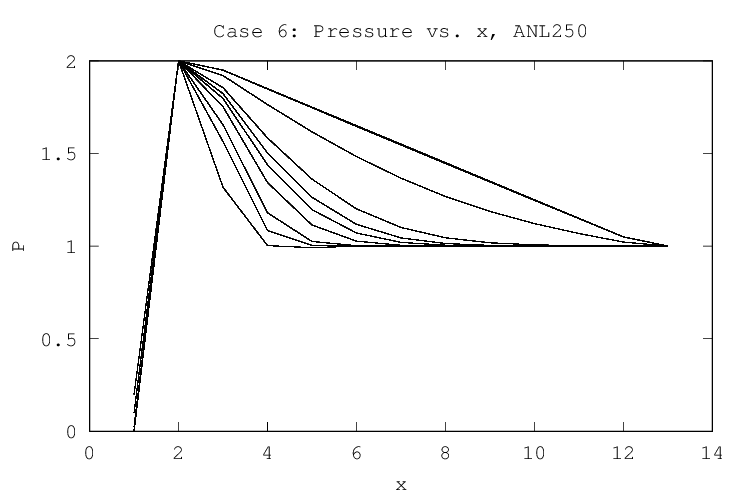
\includegraphics[]{../code/case63.png}
  \caption{Case 6, analytical solution.}
  \label{fig:case63}
\end{figure}

% subsection plots (end)
\pagebreak

\subsection{Listings} % (fold)
\label{sub:listings}

\lstinputlisting[%
  caption={Main program},
  label={lst:mainprog},
  language={[90]Fortran}]
  {../code/MainProg.f90}

\lstinputlisting[%
  caption={Shell script for data set generation},
  label={lst:shellscript},
  language={sh}]
  {../code/GenerateData.sh}

  \pagebreak

\lstinputlisting[%
  caption={Matlab script for plot generation},
  label={lst:plotgen},
  language={Matlab}]
  {../code/GeneratePlots.m}
% subsection listings (end)


% section fortran_program (end)
  
\end{document}
